\section{Giai đoạn 2: Phân tích cú pháp phân cấp, chuẩn hóa và khử trùng lặp}

Sau khi Giai đoạn 1 hoàn tất thu thập lịch sử phiên bản và trích xuất chọn lọc mã nguồn văn bản cùng thư mục tham khảo cho $25{,}000$ bài báo, Giai đoạn 2 đảm nhiệm việc chuyển hóa các cây thư mục LaTeX không đồng nhất thành biểu diễn quan hệ có cấu trúc gồm ba bảng đầu ra: bảng phần tử nội dung, bảng quan hệ phân cấp và bảng mục lục BibTeX hợp nhất \cite{hcmus_intro_ds}. Quá trình chuyển hóa trên dữ liệu arXiv thực tế phải giải quyết đồng thời ba thách thức kỹ thuật giao thoa. Thứ nhất, các gói nguồn thường phân mảnh qua nhiều thư mục lồng nhau, xen lẫn bản nháp bị chú thích hóa, tệp mẫu của nhà xuất bản và tài liệu con độc lập. Thứ hai, việc chạy trình biên dịch TeX đầy đủ không khả thi về thời gian lẫn độ an toàn trước các lệnh tự định nghĩa tùy biến, đòi hỏi kiến trúc phân tích cú pháp bảo toàn và có tính tất định. Thứ ba, do $42.64\%$ bài báo trong kho có từ hai phiên bản trở lên, việc lưu trữ rời rạc từng phiên bản sẽ làm phình dung lượng và lặp dữ liệu văn bản nghiêm trọng. Thiết kế Giai đoạn 2 do đó gắn chặt việc gom tệp theo đường biên dịch, hợp nhất khóa trích dẫn sớm, tách câu không dùng chuỗi giữ chỗ và khử trùng lặp hai mức vào một dây chuyền liên kết thống nhất.

\subsection{Gom tệp theo đường biên dịch và thứ tự xử lý liên giai đoạn}

Một bản nộp arXiv điển hình là một cây thư mục phức hợp phản ánh trực tiếp quy trình soạn thảo của nhóm tác giả. Bên trong cùng một phiên bản thường tồn tại đồng thời tệp bản thảo chính, nhiều tệp chương mục con, tệp hình vẽ biên dịch độc lập, bản sao lưu cũ trong thư mục phụ, tệp xem trước tạm của trình soạn thảo và cả các tệp thư mục tham khảo mẫu không hề được trích dẫn. Việc ghép cơ học toàn bộ tệp nguồn theo thứ tự bảng chữ cái trên đĩa sẽ làm đảo lộn cấu trúc lập luận, đưa nội dung thừa vào văn bản chính và làm hỏng cây phân cấp ở công đoạn tiếp theo. Để xử lý an toàn, thành phần quét cây thư mục đọc tệp bằng mã hóa UTF-8 kèm dự phòng Latin-1, chuẩn hóa dấu xuống dòng, bỏ qua liên kết tượng trưng và chặn mọi đường dẫn thoát khỏi thư mục gốc của phiên bản. Trước khi phân tích lệnh cấu trúc, mỗi tệp nguồn được đưa qua bộ che chú thích bảo toàn độ lệch ký tự. Bộ quét đếm số dấu gạch chéo ngược đứng liền trước từng ký tự phần trăm để phân biệt ký tự phần trăm thoát mang nghĩa văn bản (số dấu gạch chéo lẻ) với dấu mở chú thích hoạt động (số dấu gạch chéo chẵn), sau đó thay toàn bộ phần chú thích bằng khoảng trắng cùng độ dài nhằm vô hiệu hóa lệnh ẩn mà không làm xê dịch bất kỳ chỉ số ký tự nào.

Bước quyết định tiếp theo là định danh tệp nguồn gốc mà trình biên dịch LaTeX thực sự khởi chạy từ đó, áp dụng trên tập các ứng viên chứa lệnh khai báo lớp tài liệu không bị chú thích hóa. Thay vì dựa vào tên tệp cố định vốn dễ thất bại trên các gói nộp phi quy ước, hệ thống xếp hạng mọi ứng viên $p$ theo khóa thứ tự từ điển chín tiêu chí và chọn ứng viên nhỏ nhất:
\begin{equation}
    K(p) = \bigl(k_1(p),\, k_2(p),\, k_3(p),\, k_4(p),\, k_5(p),\, k_6(p),\, -L_{\text{exp}}(p),\, d(p),\, p\bigr).
    \label{eq:m2_root_rank}
\end{equation}
Trong Phương trình~\eqref{eq:m2_root_rank}, sáu thành phần đầu là các chỉ báo nhị phân thuộc $\{0, 1\}$ với giá trị $0$ biểu thị mức ưu tiên cao hơn: $k_1$ loại trừ tệp tạm xem trước do trình soạn thảo tạo ra, $k_2$ yêu cầu có phần thân tài liệu mở thực sự và $k_3$ hạ bậc các lớp tài liệu đóng gói hình vẽ độc lập hoặc tài liệu con. Ba tiêu chí nhị phân kế tiếp kiểm tra quan hệ cấu trúc và quy ước lưu trữ: $k_4$ ưu tiên tệp không bị bất kỳ tệp đồng cấp nào khác nạp vào, $k_5$ ưu tiên tệp đặt trực tiếp ở thư mục cấp cao nhất thay vì bản sao lưu trong thư mục con và $k_6$ ưu tiên các tên bản thảo quy ước phổ biến. Khi nhiều ứng viên bằng nhau ở cả sáu tiêu chí này, thành phần thứ bảy $-L_{\text{exp}}(p)$ chọn tệp cho tổng độ dài ký tự sau khi bung toàn bộ đường dẫn nạp lớn nhất. Hai thành phần cuối cùng sử dụng độ sâu thư mục $d(p)$ và thứ tự từ điển của đường dẫn $p$ để bảo đảm kết quả lựa chọn luôn duy nhất và tất định.

Từ tệp gốc đã xác định, bộ mở rộng đệ quy thực hiện bung bắc cầu mọi chỉ thị nạp tệp theo đúng thứ tự biên dịch thực tế. Hệ thống phân giải đường dẫn đích theo trình tự thư mục chứa tệp gốc, kế đến là thư mục chứa tệp đang gọi lệnh nạp nhằm tương thích với dự án soạn thảo trực tuyến, rồi mới tới thư mục gốc của gói nộp, luôn ưu tiên khớp hoa thường tuyệt đối trước khớp không phân biệt hoa thường. Khi gặp chỉ thị nạp tài liệu con độc lập, bộ mở rộng chỉ cắt lấy phần thân tài liệu bên trong cặp mở--đóng phần thân và bỏ qua tiền sảnh trùng lặp của tệp con. Khi gặp chỉ thị kết thúc nhập liệu sớm, phần văn bản phía sau trong tệp hiện hành lập tức bị cắt bỏ, đồng thời các định nghĩa chuỗi đường dẫn không tham số khai báo trước đó trong vùng mã hoạt động được thay thế động trước lúc phân giải đường dẫn. Nhằm ngăn vòng lặp vô hạn và tràn ngăn xếp, hệ thống kiểm tra chu trình trên ngăn xếp nạp hiện hành kết hợp giới hạn độ sâu đệ quy tối đa $D_{\max} = 64$, tự động loại bỏ nhánh tạo chu trình và ghi nhận nhật ký chẩn đoán. Trường hợp phụ thuộc hình thoi khi cùng một tệp hợp lệ được nạp ở nhiều vị trí không tạo chu trình sẽ được nhúng đầy đủ tại mỗi điểm gọi như trình biên dịch thực nhưng chỉ ghi nhận một lần trong danh mục đường biên dịch, kèm ký tự xuống dòng cuối mỗi đoạn nhúng để dòng chú thích cuối tệp con không nuốt nội dung phía sau. Cuối cùng, việc tìm kiếm tệp thư mục BibTeX chỉ căn cứ nghiêm ngặt trên các lệnh khai báo thư mục hoạt động trong văn bản đã hợp nhất thay vì quét đĩa, giúp loại bỏ hoàn toàn các tệp thư mục mẫu dư thừa.

\begin{figure}[H]
    \centering
    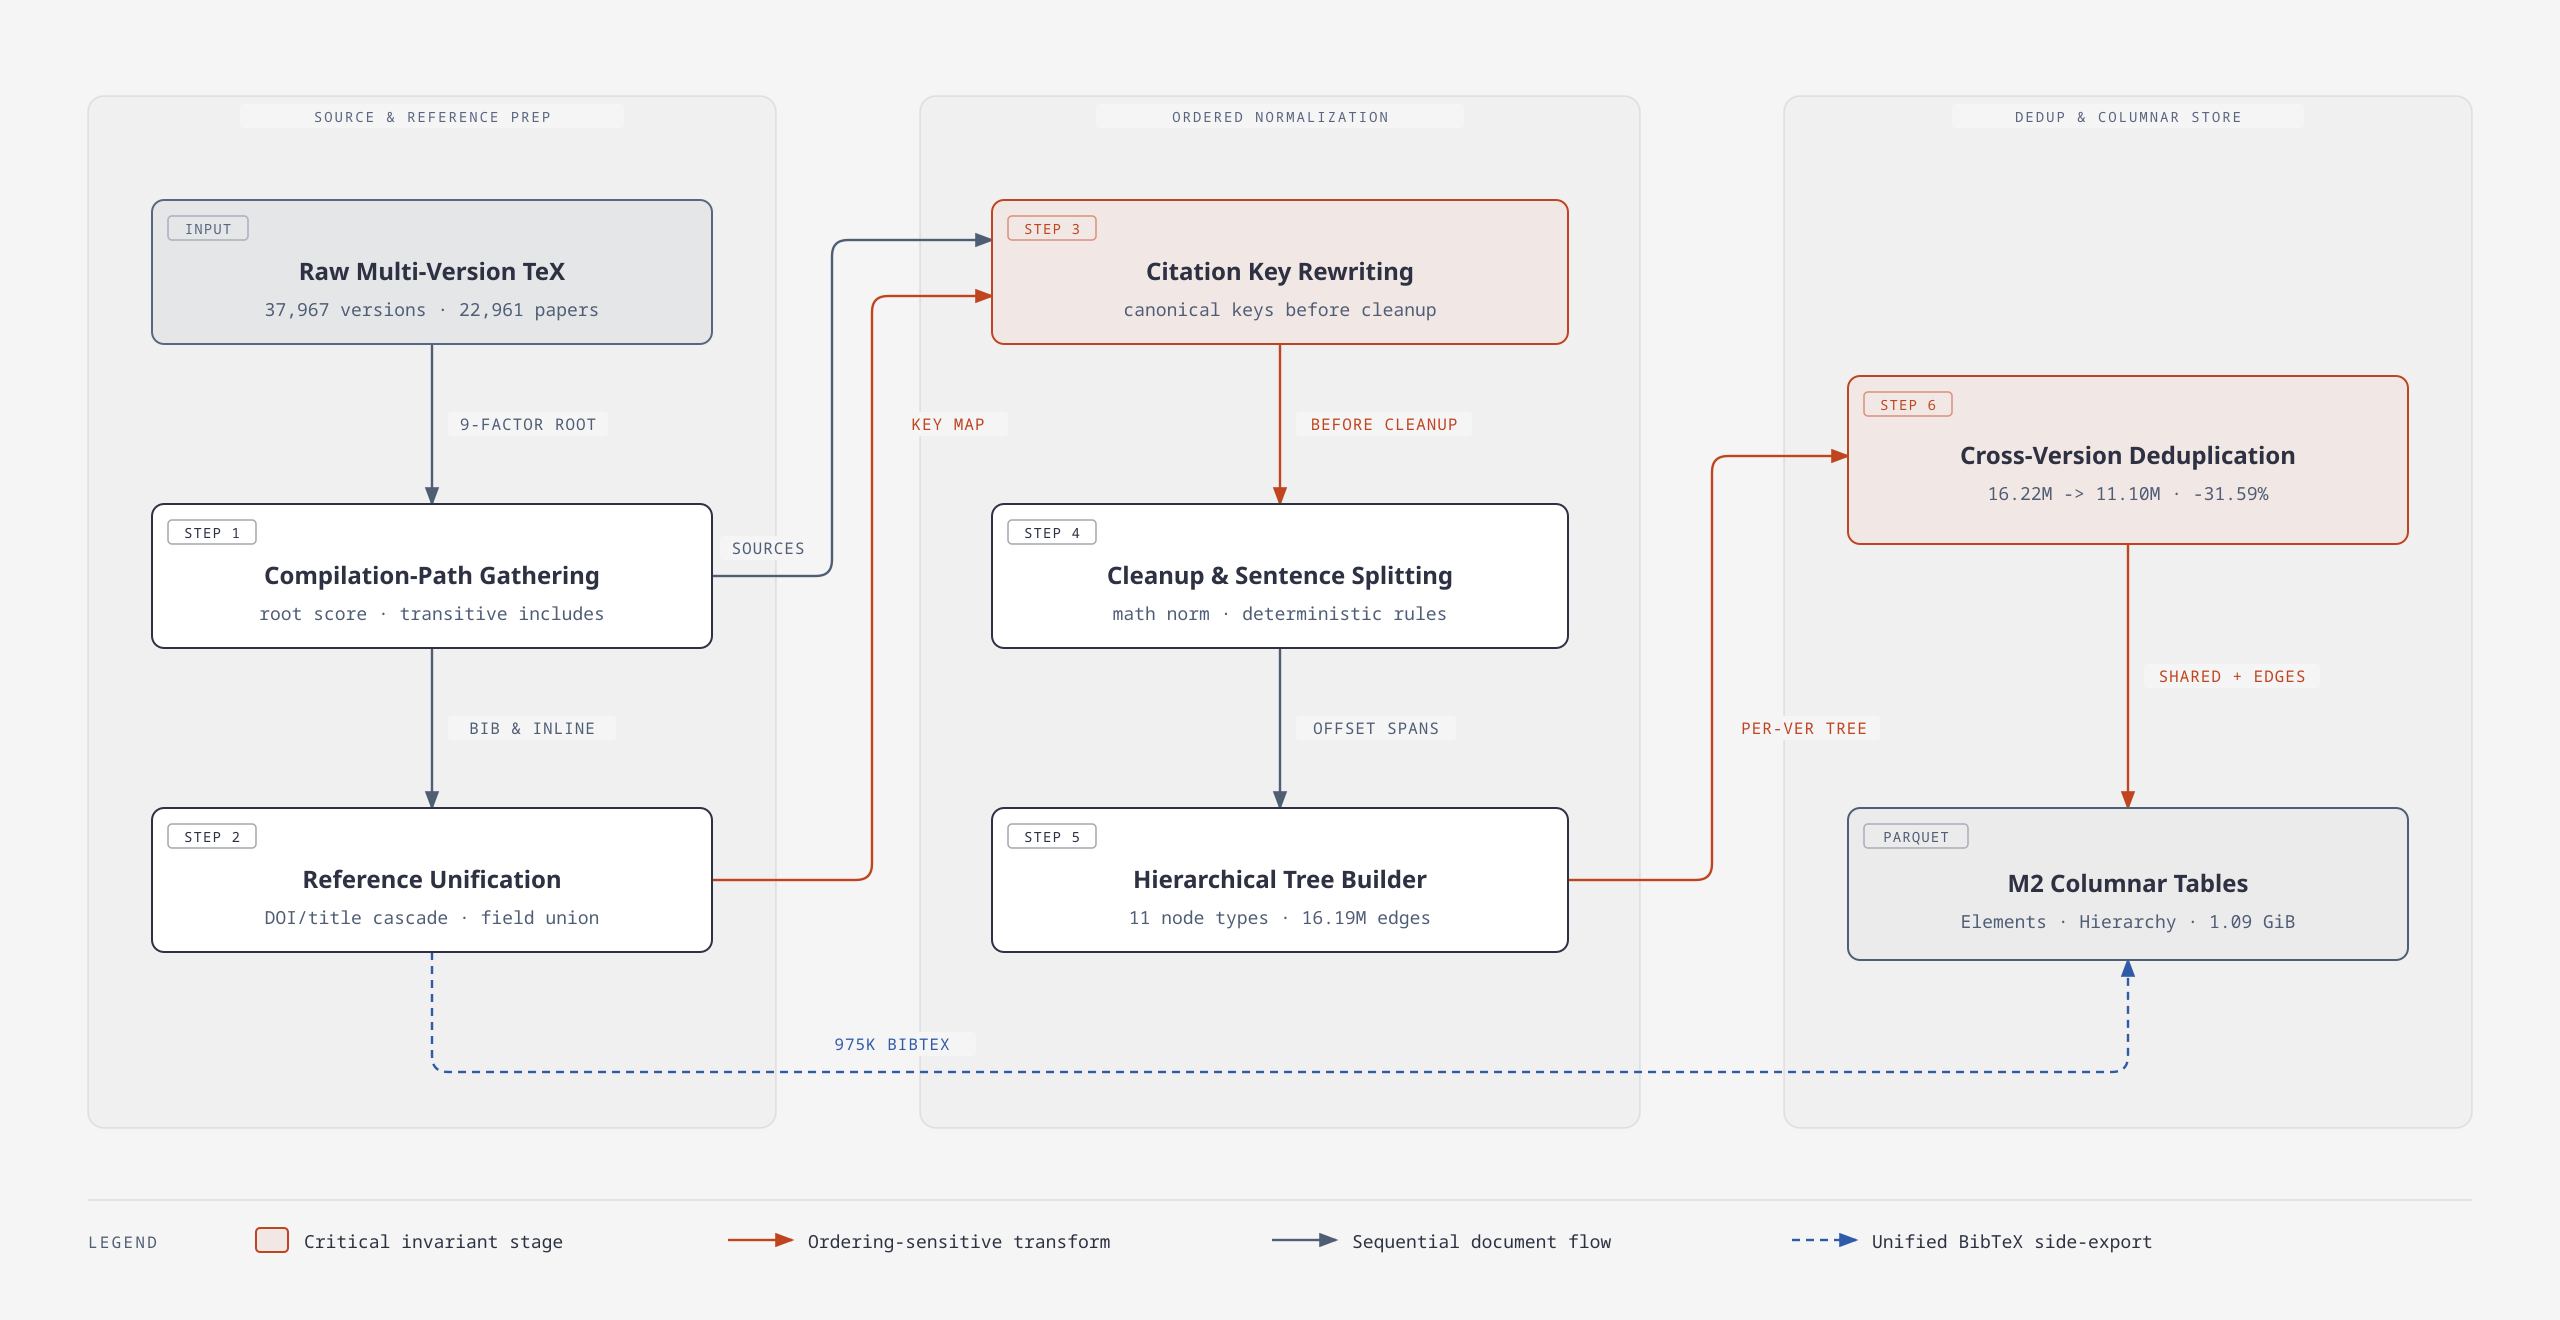
\includegraphics[width=\linewidth]{images/m2_parsing_dedup.png}
    \caption[Kiến trúc xử lý liên giai đoạn và khử trùng lặp của Giai đoạn 2]{Kiến trúc xử lý liên giai đoạn của Giai đoạn 2: gom tệp theo đường biên dịch, trích xuất và viết lại khóa trích dẫn trước khi dựng cây phân cấp, chuẩn hóa không chuỗi giữ chỗ và khử trùng lặp nội dung liên phiên bản.}
    \label{fig:m2_parsing_dedup}
\end{figure}

Một quyết định kiến trúc mang tính bản lề của Giai đoạn 2 nằm ở \textbf{thứ tự xử lý liên giai đoạn} giữa trích xuất thư mục tham khảo và dựng cây nội dung, được minh họa trong Hình~\ref{fig:m2_parsing_dedup}. Nếu dựng cây phân cấp, tách câu và băm khử trùng lặp trước rồi mới hợp nhất tài liệu tham khảo sau, hệ thống sẽ gặp lỗi lệch khóa trên các bài báo đa phiên bản. Cụ thể, khi tác giả đổi tên khóa trích dẫn của cùng một bài tham khảo giữa hai phiên bản nhưng giữ nguyên toàn bộ câu văn xuôi, hai câu hoàn toàn tương đương về ngữ nghĩa sẽ mang chuỗi khóa khác nhau và thất bại khi đối sánh khử trùng lặp toàn văn. Đồng thời, các lệnh trích dẫn còn lưu trong bảng phần tử nội dung sẽ không khớp với khóa chuẩn trong bảng mục lục BibTeX hợp nhất. Vì vậy, dây chuyền đảo ngược thứ tự xử lý: ngay sau bước gom tệp đa nguồn cho mọi phiên bản của một bài báo, thành phần trích xuất và hợp nhất thư mục tham khảo chạy trước tiên để ánh xạ mọi khóa cục bộ về khóa chuẩn và viết lại trực tiếp các lệnh trích dẫn trong luồng nguồn của từng phiên bản. Chỉ sau khi khóa chuẩn đã lan truyền đồng bộ vào toàn bộ văn bản, các bước dựng cây phân cấp, làm sạch LaTeX, chuẩn hóa toán học, tách câu và khử trùng lặp nội dung mới được thực thi.

\subsection{Dựng cây phân cấp tự động, chuẩn hóa và tách câu theo lát cắt bù trừ}

Trên luồng mã nguồn đã đồng bộ khóa trích dẫn của từng phiên bản, bộ dựng cây cấu trúc tự động loại bỏ chú thích dòng, các môi trường chú thích lồng nhau (trong khi giữ nguyên các khối mã nguyên văn) cùng các khai báo định nghĩa lệnh tùy biến trong phần thân để phần thân lệnh không sinh ra tiêu đề mục giả. Bộ quét luồng sau đó duyệt tuyến tính qua phần thân tài liệu và duy trì một ngăn xếp phạm vi phân cấp nhằm gán nút cha hiện hành cho từng thành phần mới. Ngăn xếp khởi đầu bằng nút gốc phiên bản tài liệu ở độ sâu $0$, tiếp nối bởi năm cấp tiêu đề giảm dần gồm chương, mục chính, tiểu mục cấp hai, tiểu mục cấp ba và tiêu đề đoạn văn (độ sâu từ $1$ đến $5$, trong đó cấp chương được quy về loại mục chính để giữ nhất quán lược đồ). Đối với danh sách có thứ tự và không thứ tự, khung danh sách nhận độ sâu bằng độ sâu nút cha cộng $10$ và mỗi mục con bên trong nhận độ sâu cộng thêm $1$, nhờ đó hỗ trợ danh sách lồng nhau nhiều tầng mà không xung đột cấp bậc với cấu trúc mục. Ở tầng thấp nhất, cây phân cấp chỉ chấp nhận nghiêm ngặt ba loại nút lá kết thúc không bao giờ đẩy vào ngăn xếp: câu văn xuôi, công thức toán học dạng khối và hình vẽ (hợp nhất cả hình ảnh, bảng dữ liệu, hình bảng bao văn bản và bảng nhiều trang về cùng loại nút lá hình vẽ theo đặc tả \cite{hcmus_intro_ds}).

Cơ chế tháo ngăn xếp tự động giúp bộ dựng cây thích ứng bền vững với cấu trúc soạn thảo phi chuẩn trong kho tiền ấn. Khi gặp một tiêu đề mới ở cấp $\ell$, ngăn xếp tự động bật bỏ mọi khung đang mở có độ sâu lớn hơn hoặc bằng $\ell$ nhưng luôn dừng lại trước nút gốc độ sâu $0$. Nhờ quy tắc này, các bài báo nhảy cấp trực tiếp từ mục chính xuống tiểu mục cấp ba hoặc bỏ quên lệnh đóng danh sách trước khi mở mục mới vẫn sinh cây hợp lệ. Tương tự, các lệnh đóng danh sách mồ côi sẽ bị bỏ qua an toàn nếu không tồn tại khung danh sách tương ứng trên ngăn xếp. Về phạm vi chọn lọc, mọi mục mang tiêu đề tham khảo đã chuẩn hóa cùng các môi trường hoặc chỉ thị danh mục tài liệu tham khảo đều bị loại trừ; ngược lại, mục lời cảm ơn không đánh số vẫn được giữ như mục bình thường, và chỉ thị phụ lục sau danh mục tham khảo lập tức đặt lại cờ loại trừ để bảo toàn trọn vẹn nội dung phụ lục. Sau khi quét xong, mọi cây phiên bản đều đi qua trình kiểm định tự động sáu bất biến cấu trúc: cho phép cây rỗng với phiên bản thiếu nguồn TeX, bắt buộc đúng một nút gốc không cha thuộc loại tài liệu với cây không rỗng, mọi liên kết cha phải trỏ tới nút tồn tại trong cùng phiên bản, mã định danh tạm phải duy nhất, loại nút phải thuộc tập từ vựng đóng và đồ thị cha--con tuyệt đối không chứa chu trình.

Song song với phân tích cấu trúc, nội dung văn bản và công thức đi qua bộ chuẩn hóa LaTeX bảo toàn một lượt quét. Thiết kế này xuất phát từ đánh đổi kỹ thuật cốt lõi: thực thi TeX đầy đủ quá tốn kém và kém an toàn với lệnh tự định nghĩa, còn việc xóa thô bằng biểu thức chính quy dễ phá hủy biểu thức toán và ký hiệu mảng trong ngoặc vuông. Do đó, bộ làm sạch bỏ qua nguyên vẹn mọi vùng toán học và giữ lại mọi lệnh chuyên ngành chưa rõ ngữ nghĩa, chỉ loại bỏ các chỉ thị trình bày phi ngữ nghĩa như căn chỉnh, ngắt trang, đường kẻ bảng ngang, khoảng trắng đứng ngang, cỡ chữ, gán thanh ghi độ dài hay bộ đếm đủ số đối số, gán thụt lề và khai báo định nghĩa lệnh. Các lệnh nhấn mạnh văn xuôi như in đậm, in nghiêng, gạch chân cùng các lớp bọc bố cục hai cột hoặc co giãn tỷ lệ được bóc vỏ đệ quy để bảo toàn nội dung thuần bên trong, áp dụng tương tự cho chú thích hình và bảng. Đặc biệt, thao tác xóa tùy chọn đặt vị trí hình nổi được thiết kế theo ngữ cảnh, chỉ kích hoạt ngay sau thẻ mở môi trường hình hoặc bảng nhằm bảo toàn tuyệt đối ký hiệu khoảng đóng và chỉ số mảng đặt trong ngoặc vuông giữa văn xuôi. Tiếp đó, bộ chuẩn hóa công thức toán kiểm tra tính chẵn lẻ dấu gạch chéo ngược để không nhận nhầm ký hiệu tiền tệ thoát hay lệnh xuống dòng, đưa mọi công thức nội tuyến về cặp dấu đô-la đơn và thống nhất toàn bộ công thức khối (cặp dấu đô-la kép, ngoặc vuông khối, cùng các môi trường phương trình, căn hàng và nhóm công thức có hoặc không đánh số) về khối phương trình chuẩn duy nhất.

Ở bước tách khối văn xuôi thành từng câu, kỹ thuật truyền thống thường thay thế công thức toán, lệnh LaTeX và địa chỉ mạng bằng các mã thẻ giữ chỗ nhân tạo trước khi đưa qua bộ tách câu, rồi đối sánh chuỗi để ghép ngược văn bản gốc. Thực tế triển khai trên văn bản khoa học bộc lộ điểm yếu nghiêm trọng của phương pháp này: khi bộ tách câu thống kê hoặc mạng nơ-ron tự chỉnh sửa khoảng trắng, tách dấu câu kề mã thẻ hoặc gặp cấu trúc ngoặc lồng nhau bên cạnh công thức, một số mã thẻ không thể khớp ngược và rò rỉ vĩnh viễn vào dữ liệu đầu ra. Hiện tượng này còn gây lệch ranh giới câu âm thầm, làm biến dạng nội dung toán học và phá vỡ phép so khớp khử trùng lặp giữa các phiên bản. Trên quy mô hơn $8.6$ triệu câu của kho dữ liệu, ngay cả tỷ lệ rò rỉ $0.1\%$ cũng đủ đưa hàng nghìn chuỗi lỗi vào bảng phần tử nội dung. Vì vậy, bài toán đòi hỏi một cơ chế bảo vệ cú pháp không can thiệp vào chuỗi gốc và loại bỏ hoàn toàn bước thay thế ngược.

Để giải quyết triệt để vấn đề trên, nhóm thiết kế kiến trúc \textbf{tách câu theo lát cắt bù trừ không dùng chuỗi giữ chỗ} dùng chung cho mọi bộ tách câu. Với đoạn văn xuôi đã làm sạch $T$ dài $n$ ký tự, bộ quét tuyến tính một lượt xác định tập khoảng bảo vệ rời nhau $\mathcal{P} = \{[a_k, b_k)\}_{k=1}^{m}$ bao phủ vùng toán học nội tuyến và khối, đối số ngoặc cân bằng của lệnh LaTeX, danh mục $20$ chữ viết tắt học thuật không phân biệt hoa thường (nhận diện cả khoảng trắng thường lẫn khoảng trống mỏng của TeX bên trong mà không nuốt khoảng trắng sau dấu chấm cuối), số thập phân cùng số hiệu phiên bản, địa chỉ thư điện tử và địa chỉ mạng có bảo toàn ngoặc cân bằng (chừa dấu chấm kết câu bên ngoài nhưng giữ ngoặc đóng cân bằng bên trong đường dẫn). Từ $\mathcal{P}$, hệ thống tạo hình chiếu che $M$ cùng độ dài tuyệt đối $|M| = |T| = n$:
\begin{equation}
    M[i] =
    \begin{cases}
        T[i] & \text{nếu } i \notin \bigcup_{k=1}^{m} [a_k, b_k) \text{ hoặc } T[i] \text{ là khoảng trắng}, \\
        \text{ký tự chữ cái trung tính} & \text{nếu } i \in \bigcup_{k=1}^{m} [a_k, b_k) \text{ và } T[i] \text{ không phải khoảng trắng}.
    \end{cases}
    \label{eq:m2_masked_view}
\end{equation}
Theo Phương trình~\eqref{eq:m2_masked_view}, hình chiếu $M$ bảo toàn chính xác từng tọa độ ký tự và mọi khoảng trắng của $T$, cho phép mọi bộ tách câu chỉ cần dự đoán tập vị trí kết thúc câu $\{e_j\}$ trên $M$. Các ranh giới ứng viên sau đó đi qua lớp hậu kiểm: gắn dấu ngoặc và ngoặc kép đóng liền kề về câu trước, hủy bỏ mọi vị trí cắt nằm bên trong khoảng thuộc $\mathcal{P}$ hoặc không đứng trước khoảng trắng hay cuối đoạn, và chỉ nhận ranh giới kết thúc bằng dấu chấm. Từng câu kết quả được trích xuất trực tiếp bằng lát cắt $T[s_j : e_j]$ trên chuỗi gốc nguyên vẹn $T$, triệt tiêu hoàn toàn nguy cơ rò rỉ chuỗi giữ chỗ hay sai lệch cú pháp LaTeX.

\subsection{Thực nghiệm so sánh các bộ tách câu trên CPU và quyết định lựa chọn}

Nhờ giao diện lát cắt bù trừ độc lập với thuật toán nhận diện ranh giới, nhóm tiến hành thực nghiệm so sánh có kiểm soát hai giai đoạn trên cùng máy CPU cục bộ (Intel Core i5-8365U 4 nhân 8 luồng, Python 3.12.13) đối với bốn bộ tách câu: bộ quy tắc kèm từ điển $20$ chữ viết tắt, bộ phát hiện không giám sát NLTK Punkt \cite{kiss2006}, mô hình nhận diện câu mạng nơ-ron cỡ nhỏ tiếng Anh của spaCy \cite{spacy}, và mô hình Segment Any Text ba tầng gọn nhẹ chạy trên bộ thực thi ONNX CPU \cite{frohmann2024}. Ở Giai đoạn 1, nhóm khảo sát $11$ bài báo TeX gồm $1{,}574$ khối văn xuôi, đánh giá đồng thời độ chính xác trên $12$ trường hợp biên khó tuyển chọn (như tên viết tắt tác giả, viết tắt học thuật hiếm ngoài từ điển và dấu câu kề ngoặc) cùng $40$ bài kiểm thử tương thích hợp đồng cú pháp. Kết quả ở phần trên của Bảng~\ref{tab:m2_tokenizer_study} chỉ ra sự đánh đổi rõ rệt giữa nhận diện ngữ cảnh và kỷ luật cấu trúc. Hai mô hình mạng nơ-ron nâng điểm chẩn đoán biên khó từ $7/12$ (bộ quy tắc) và $8/12$ (Punkt) lên $10/12$ (spaCy) và $9/12$ (Segment Any Text) nhờ khái quát tốt tên viết tắt ngoài từ điển. Ngược lại, tỷ lệ tuân thủ hợp đồng giảm từ $40/40$ ở bộ quy tắc xuống $38/40$ ở Punkt, $35/40$ ở spaCy và $27/40$ ở Segment Any Text do các mô hình học máy thỉnh thoảng gộp câu qua vùng chữ cái che kỹ thuật, trong khi Segment Any Text đã tiêu tốn $222.13\text{ s}$ chỉ trên $11$ bài báo.

\begin{table}[H]
    \centering
    \footnotesize
    \setlength{\tabcolsep}{4pt}
    \renewcommand{\arraystretch}{1.22}
    \begin{tabularx}{\textwidth}{@{}X c c r r@{}}
        \toprule
        \multicolumn{5}{@{}l@{}}{\textbf{(a) Nghiên cứu chẩn đoán và hồi quy trên 11 bài báo TeX (1,574 khối văn xuôi)}} \\
        \midrule
        \textbf{Bộ tách câu} & \textbf{Chẩn đoán (/12)} & \textbf{Hợp đồng (/40)} & \textbf{Số câu tách} & \textbf{Thời gian (s)} \\
        \midrule
        Quy tắc + từ điển 20 viết tắt & 7 / 12 & \textbf{40 / 40} & 5,635 & \textbf{0.54 -- 0.80} \\
        NLTK Punkt \cite{kiss2006} & 8 / 12 & 38 / 40 & 5,630 & 0.79 \\
        spaCy mạng nơ-ron \cite{spacy} & \textbf{10 / 12} & 35 / 40 & 5,608 & 3.37 \\
        Segment Any Text (ONNX CPU) \cite{frohmann2024} & 9 / 12 & 27 / 40 & 5,466 & 222.13 \\
        \bottomrule
    \end{tabularx}

    \vspace{0.8em}

    \begin{tabularx}{\textwidth}{@{}X r r r r r@{}}
        \toprule
        \multicolumn{6}{@{}l@{}}{\textbf{(b) Đo hiệu năng hệ thống trên dải 100 mã bài CPU (93 bài TeX, 7,525 khối, 4.80 triệu ký tự)}} \\
        \midrule
        \textbf{Cấu hình mô hình nơ-ron} & \textbf{Tổng (s)} & \textbf{s / pb} & \textbf{RAM (MiB)} & \textbf{Thông lượng} & \textbf{Ước tính 40k pb} \\
        \midrule
        spaCy (cỡ lô 1) \cite{spacy} & 17.28 & 0.186 & \textbf{151.5} & 278k ký tự/s & 2.06 giờ \\
        spaCy (cỡ lô 32) \cite{spacy} & \textbf{9.70} & \textbf{0.104} & 163.6 & \textbf{495k ký tự/s} & \textbf{1.16 giờ} \\
        Segment Any Text (cỡ lô 1) \cite{frohmann2024} & 1,283.91 & 13.805 & 1,310.1 & 3.74k ký tự/s & 153.39 giờ \\
        \bottomrule
    \end{tabularx}
    \caption[So sánh thực nghiệm bốn bộ tách câu trên môi trường CPU cục bộ]{Kết quả thực nghiệm so sánh bốn bộ tách câu trên cùng môi trường CPU cục bộ (Intel Core i5-8365U 4 nhân 8 luồng, Python 3.12.13). Ở thử nghiệm dải 100 mã bài, 6 bài chỉ có PDF và 1 bài vượt ngưỡng thời gian chờ; công đoạn chuẩn bị kho văn bản (giải nén, gom tệp, làm sạch và quét cấu trúc) tiêu tốn 35.89 s.}
    \label{tab:m2_tokenizer_study}
\end{table}

Nhằm đo đạc khả năng mở rộng thực tế ở quy mô hàng chục nghìn phiên bản, Giai đoạn 2 triển khai phép đo hệ thống trên một dải $100$ mã bài liên tiếp. Dải đo chứa $93$ bài có nguồn TeX hợp lệ (gồm $7{,}525$ khối văn xuôi với $4{,}803{,}251$ ký tự), $6$ bài chỉ có PDF và $1$ bài quá hạn thời gian chờ; riêng bước chuẩn bị văn bản đầu vào mất $35.89\text{ s}$. Theo phần dưới của Bảng~\ref{tab:m2_tokenizer_study}, spaCy chạy đơn lẻ ở cỡ lô $1$ hoàn thành trong $17.28\text{ s}$ ($0.186\text{ s}$ mỗi phiên bản, bộ nhớ đỉnh $151.5\text{ MiB}$, thông lượng $278\text{ nghìn ký tự/s}$), tương ứng $2.06\text{ giờ}$ ngoại suy cho $40{,}000$ phiên bản. Khi bật gom lô cỡ $32$, spaCy tăng thông lượng $1.78$ lần lên $495\text{ nghìn ký tự/s}$ và giảm thời gian còn $9.70\text{ s}$ ($0.104\text{ s}$ mỗi phiên bản, bộ nhớ đỉnh $163.6\text{ MiB}$, ngoại suy $1.16\text{ giờ}$ cho $40{,}000$ phiên bản). Trái lại, Segment Any Text trên CPU cần tới $1{,}283.91\text{ s}$ ($13.805\text{ s}$ mỗi phiên bản, thông lượng chỉ $3.74\text{ nghìn ký tự/s}$) và chiếm $1{,}310.1\text{ MiB}$ bộ nhớ đỉnh. Mức tiêu thụ này chậm hơn $74.3\times$ so với spaCy cỡ lô $1$, chậm hơn $132.4\times$ so với spaCy cỡ lô $32$ và ngốn bộ nhớ gấp $8.0\times$ đến $8.6\times$, đẩy ước lượng $40{,}000$ phiên bản lên $153.39\text{ giờ}$ và hoàn toàn bất khả thi trên Google Colab CPU.

Dựa trên số liệu thực nghiệm hai giai đoạn, nhóm lựa chọn \textbf{bộ tách câu theo quy tắc kèm từ điển $20$ chữ viết tắt} cho toàn bộ lượt chạy sản xuất $25{,}000$ bài báo trên Google Colab CPU, đồng thời giữ nguyên spaCy gom lô và Segment Any Text như các lựa chọn cấu hình cho nghiên cứu mở rộng. Dù spaCy cỡ lô $32$ đạt điểm chẩn đoán biên khó cao hơn ($10/12$) với chi phí ngoại suy chấp nhận được ($1.16\text{ giờ}$), bộ quy tắc vượt trội về độ tin cậy vận hành trên hạ tầng đám mây phân tán của năm thành viên. Trước hết, bộ quy tắc không yêu cầu tải trọng số mô hình ngoài nên loại bỏ hoàn toàn chi phí cài đặt môi trường và nguy cơ sai khác phiên bản mô hình khi phiên Colab khởi động lại. Thứ hai, bộ quy tắc đạt độ tuân thủ tuyệt đối $40/40$ với hợp đồng cấu trúc và bảo đảm tính tất định từng bit, giúp dấu vân tay kiểm chứng điểm phục hồi luôn khớp chính xác qua các lượt chạy nối tiếp. Cuối cùng, chi phí CPU và bộ nhớ không đáng kể của bộ quy tắc giữ ổn định dung lượng RAM cho tiến trình ghi điểm phục hồi quan hệ và xuất tệp cột Parquet trên máy ảo hai nhân xử lý.

\subsection{Trích xuất thư mục tham khảo và khử trùng lặp hai mức liên phiên bản}

Chiến lược khử trùng lặp trong Giai đoạn 2 gồm hai tầng nối tiếp: \textbf{Mức 1} trích xuất và hợp nhất thư mục tham khảo liên phiên bản trước khi phân tích văn bản, và \textbf{Mức 2} khử trùng lặp toàn văn các phần tử cấu trúc cùng nút lá sau khi chuẩn hóa. Ở Mức 1, bộ trích xuất xử lý đồng thời ba định dạng thư mục phổ biến trong kho arXiv. Với các tệp BibTeX bên ngoài được gọi từ văn bản hoạt động, bộ phân tích đếm cân bằng ngoặc nhọn và ngoặc tròn, hỗ trợ mở rộng định nghĩa chuỗi văn bản kèm phép nối chuỗi, bỏ qua khối tiền sảnh hay chú thích nhưng chỉ lược bỏ ký tự phần trăm chú thích \emph{giữa} các mục để không bao giờ cắt cụt ký tự mã hóa phần trăm bên trong địa chỉ URL. Với các mục tham khảo nội tuyến trong khối danh mục tài liệu tham khảo (gồm cả môi trường chuẩn lẫn chỉ thị gọi trực tiếp), hệ thống phối hợp dấu phân cách khối, trích xuất tiêu đề trong ngoặc kép LaTeX hoặc ngoặc cong, nhận diện tên tác giả có chữ cái đầu nối gạch ngang và định dạng họ đặt trước, bảo toàn tên nhóm hợp tác khoa học trong ngoặc vuông đi kèm dạng tác giả rút gọn và giải mã dấu phụ TeX về Unicode NFC. Đặc biệt, bộ trích xuất năm công bố bốn chữ số lọc bỏ vùng URL và DOI trước khi quét, đồng thời loại trừ mọi chuỗi bốn chữ số đứng liền trước dấu chấm thập phân để không nhận nhầm mã định danh arXiv hiện đại thành năm xuất bản. Ngoài ra, bộ trích xuất còn hỗ trợ các khối thư mục chuẩn AMSRefs với trường tác giả lặp lại trong ngoặc nhọn cùng trường ngày tháng và mã bản thảo điện tử, đồng thời chỉ thu nhận những mục có khóa thực sự xuất hiện trong lệnh trích dẫn hoạt động trừ khi bản thảo yêu cầu nạp toàn bộ thư mục.

Khi hợp nhất danh sách mục tham khảo từ mọi phiên bản của một bài báo được sắp xếp theo thứ tự thời gian tăng dần, hệ thống áp dụng tầng định danh ba bước nhằm nhận diện chính xác cùng một công trình dù khóa trích dẫn hay dấu câu thay đổi giữa các lần chỉnh sửa:
\begin{equation}
    \mathcal{I}(r) =
    \begin{cases}
        \text{DOI chuẩn hóa}(r) & \text{nếu } r \text{ có DOI hợp lệ}, \\
        \text{Tiêu đề ASCII chuẩn hóa}(r) & \text{nếu } |\tilde{t}(r)| \ge 8 \text{ và } |W(\tilde{t}(r))| \ge 2, \\
        \text{Khóa trích dẫn thường hóa}(r) & \text{chỉ khi thiếu cả hai định danh trên}.
    \end{cases}
    \label{eq:m2_bib_identity}
\end{equation}
Trong Phương trình~\eqref{eq:m2_bib_identity}, DOI chuẩn hóa (chữ thường, đã lược tiền tố đường dẫn phân giải và dấu câu thừa) là căn cứ đối sánh quyết định. Tầng thứ hai dùng tiêu đề đã phân rã Unicode NFKD, gập về ký tự ASCII chữ thường chỉ giữ chữ và số, nhưng buộc đạt tối thiểu $8$ ký tự và ít nhất $2$ từ nhằm tránh gộp nhầm các chuỗi ngắn chung chung. Tầng thứ ba chỉ kích hoạt khi thiếu cả DOI lẫn tiêu đề đáng tin cậy. Để ngăn gộp sai và hỏng đồ thị trích dẫn, thuật toán thi hành đồng bộ bốn rào chắn an toàn: một bản ghi thiếu DOI không được phép bắc cầu nối hai mục chuẩn mang hai DOI khác nhau; nếu cùng một khóa xuất hiện hai lần trong \emph{cùng một phiên bản} để chỉ hai công trình phân biệt, tầng đối sánh theo khóa bị tắt, khe khóa bị đánh dấu mơ hồ kèm nhật ký xung đột và bước viết lại trích dẫn sẽ chủ động bỏ qua khóa đó (cũng như chặn các phiên bản sau ánh xạ tới khóa từng mơ hồ ở phiên bản gốc); khóa chuẩn đầu ra luôn chọn theo phiên bản sớm nhất và tự gắn hậu tố số tất định khi hai công trình độc lập tình cờ dùng trùng khóa cục bộ; và phép gộp siêu dữ liệu thực hiện hợp không phá hủy bằng cách giữ nguyên trường đã có, điền bổ sung các trường còn thiếu và gom thêm mọi tên tác giả phân biệt mới xuất hiện. Bản đồ ánh xạ khóa sau hợp nhất lập tức được dùng để viết lại mọi lệnh trích dẫn trên luồng LaTeX của từng phiên bản trước bước dựng cây.

Sau khi toàn bộ các phiên bản của bài báo đã được viết lại khóa trích dẫn, dựng cây phân cấp, làm sạch LaTeX và chuẩn hóa toán học, cơ chế \textbf{khử trùng lặp toàn văn Mức 2} tiến hành hợp nhất nội dung trên phạm vi toàn bộ bài báo. Hệ thống duy trì một kho nội dung dùng chung cấp bài báo được lập chỉ mục theo cặp gồm loại phần tử và chuỗi văn bản đã chuẩn hóa khoảng trắng cùng dấu xuống dòng. Mỗi cặp khóa mới nhận một mã định danh chuẩn duy nhất gắn tiền tố bài báo và loại cấu trúc, đồng thời lưu đúng một dòng vào bảng phần tử nội dung; mọi lần xuất hiện trùng khớp ở các phiên bản sau tái sử dụng nguyên mã định danh chuẩn này. Tuy nhiên, bộ khử trùng lặp áp đặt hai ngoại lệ bảo toàn cấu trúc bắt buộc nhằm giữ đúng ngữ nghĩa cây phân cấp. Thứ nhất, nút gốc phiên bản tài liệu luôn giữ mã định danh riêng theo từng số phiên bản để mỗi phiên bản có điểm khởi đầu phân biệt trong đồ thị. Thứ hai, các vật chứa danh sách và mục danh sách mang nội dung khung mẫu rỗng ngữ nghĩa không bao giờ bị gộp giữa các lần xuất hiện, tránh tình trạng nhiều nhánh danh sách độc lập ở các mục khác nhau sập chung về một nút cha duy nhất.

Ở lượt duyệt thứ hai trên từng cây phiên bản, toàn bộ liên kết cha--con theo mã tạm cục bộ được ánh xạ sang cặp mã định danh chuẩn và lưu vào bảng quan hệ phân cấp kèm mã bài báo cùng số hiệu phiên bản, đồng thời loại bỏ mọi cạnh tự trỏ suy biến nếu có. Nhờ đó, bộ đếm lượt xuất hiện phần tử thô và bộ đếm phần tử duy nhất luôn đối khớp chính xác theo từng bài báo, giúp định lượng trực tiếp mức tiết kiệm dung lượng ở quy mô kho. Kiến trúc tách biệt bảng nội dung dùng chung và bảng cạnh theo phiên bản cho phép truy xuất chính xác cấu trúc nguyên vẹn của bất kỳ phiên bản nào chỉ bằng phép lọc theo số phiên bản mà không phải nhân bản văn bản. Bên cạnh đó, những phiên bản không chứa mã nguồn TeX hợp lệ được ghi nhận tường minh là phiên bản rỗng gồm không phần tử thay vì bị loại bỏ lặng lẽ khỏi đầu ra. Cơ chế ghi nhận tường minh này bảo đảm các báo cáo kiểm định luôn phân tách rõ ràng giữa độ phủ phiên bản trong kho lưu trữ và tỷ lệ phiên bản phân tích được nội dung LaTeX.

\subsection{Thống kê toàn bộ kho dữ liệu 25,000 bài báo và đánh giá dung lượng}

Kết quả vận hành Giai đoạn 2 trên toàn bộ $25{,}000$ bài báo của năm thành viên tạo nên kho dữ liệu phân cấp hoàn chỉnh với độ phủ đồng đều qua năm dải thời gian, được tổng hợp chi tiết trong Bảng~\ref{tab:m2_owner_stats}. Toàn kho đạt $22{,}961$ trên $25{,}000$ bài báo có tối thiểu một phần tử nội dung ($91.84\%$) và $2{,}039$ bài báo rỗng không có nguồn TeX ($8.16\%$). Ở cấp độ phiên bản, $37{,}967$ trên $40{,}896$ phiên bản khai báo được dựng cây thành công, tương ứng tỷ lệ phủ $92.84\%$. So với mức độ sẵn có nguồn TeX khoảng $97\%$ được ghi nhận trên arXiv \cite{ginev2024}, độ chênh khoảng $4$--$5$ điểm phần trăm bắt nguồn từ các bài chỉ nộp PDF, gói lưu trữ không hỗ trợ đã sàng lọc ở Giai đoạn 1 và tỷ lệ nhỏ gói nguồn thiếu thân tài liệu hợp lệ. Sự ổn định xuyên suốt năm dải dữ liệu được thể hiện rõ khi tỷ lệ bài phân tích thành công nằm gọn từ $90.88\%$ đến $93.28\%$ và tỷ lệ phiên bản đạt từ $92.01\%$ đến $94.08\%$. Đáng chú ý, dữ liệu xuất bản thỏa mãn tuyệt đối đẳng thức kiểm định toàn vẹn cây: $16{,}185{,}255$ cạnh phân cấp cộng với đúng $37{,}967$ nút gốc phiên bản bằng chính xác $16{,}223{,}222$ lượt xuất hiện phần tử thô trước khử trùng lặp, xác nhận không có bất kỳ nút lạc hay mất liên kết nào trên toàn hệ thống.

\begin{table}[H]
    \centering
    \footnotesize
    \setlength{\tabcolsep}{4pt}
    \renewcommand{\arraystretch}{1.18}
    \begin{tabularx}{\textwidth}{@{}X r r r r r r r@{}}
        \toprule
        \textbf{Thành viên} &
        \shortstack[r]{\textbf{Bài có TeX} \\ \textbf{(Tỷ lệ)}} &
        \shortstack[r]{\textbf{Phiên bản} \\ \textbf{(Tỷ lệ)}} &
        \shortstack[r]{\textbf{Lượt} \\ \textbf{thô}} &
        \shortstack[r]{\textbf{Duy nhất} \\ \textbf{(Giảm)}} &
        \shortstack[r]{\textbf{Cạnh} \\ \textbf{cây}} &
        \shortstack[r]{\textbf{BibTeX} \\ \textbf{(Số bài)}} &
        \shortstack[r]{\textbf{Parquet} \\ \textbf{(MiB)}} \\
        \midrule
        Trịnh Huỳnh Nhi &
            \shortstack[r]{4,578 \\ {\scriptsize (91.56\%)}} &
            \shortstack[r]{7,687 \\ {\scriptsize (92.97\%)}} &
            3,194,213 &
            \shortstack[r]{2,167,101 \\ {\scriptsize (-32.16\%)}} &
            3,186,526 &
            \shortstack[r]{195,076 \\ {\scriptsize (3,888)}} &
            217.22 \\
        \addlinespace[3pt]
        Ngô Mẫn Nhi &
            \shortstack[r]{4,544 \\ {\scriptsize (90.88\%)}} &
            \shortstack[r]{7,592 \\ {\scriptsize (92.01\%)}} &
            3,276,789 &
            \shortstack[r]{2,221,136 \\ {\scriptsize (-32.22\%)}} &
            3,269,197 &
            \shortstack[r]{195,360 \\ {\scriptsize (3,819)}} &
            222.02 \\
        \addlinespace[3pt]
        Huỳnh Huy Hoàng &
            \shortstack[r]{4,664 \\ {\scriptsize (93.28\%)}} &
            \shortstack[r]{7,888 \\ {\scriptsize (94.08\%)}} &
            3,262,182 &
            \shortstack[r]{2,198,596 \\ {\scriptsize (-32.60\%)}} &
            3,254,294 &
            \shortstack[r]{203,414 \\ {\scriptsize (3,923)}} &
            227.36 \\
        \addlinespace[3pt]
        Phạm Minh Trọng &
            \shortstack[r]{4,585 \\ {\scriptsize (91.70\%)}} &
            \shortstack[r]{7,449 \\ {\scriptsize (92.42\%)}} &
            3,334,790 &
            \shortstack[r]{2,288,312 \\ {\scriptsize (-31.38\%)}} &
            3,327,341 &
            \shortstack[r]{194,577 \\ {\scriptsize (3,868)}} &
            227.95 \\
        \addlinespace[3pt]
        Nguyễn Phúc Khang &
            \shortstack[r]{4,590 \\ {\scriptsize (91.80\%)}} &
            \shortstack[r]{7,351 \\ {\scriptsize (92.66\%)}} &
            3,155,248 &
            \shortstack[r]{2,223,044 \\ {\scriptsize (-29.54\%)}} &
            3,147,897 &
            \shortstack[r]{187,247 \\ {\scriptsize (3,706)}} &
            222.72 \\
        \midrule
        \textbf{Tổng toàn nhóm} &
            \shortstack[r]{\textbf{22,961} \\ {\scriptsize \textbf{(91.84\%)}}} &
            \shortstack[r]{\textbf{37,967} \\ {\scriptsize \textbf{(92.84\%)}}} &
            \textbf{16,223,222} &
            \shortstack[r]{\textbf{11,098,189} \\ {\scriptsize \textbf{(-31.59\%)}}} &
            \textbf{16,185,255} &
            \shortstack[r]{\textbf{975,674} \\ {\scriptsize \textbf{(19,204)}}} &
            \textbf{1,117.27} \\
        \bottomrule
    \end{tabularx}
    \caption{Thống kê kết quả phân tích cú pháp, khử trùng lặp, trích xuất thư mục tham khảo và dung lượng lưu trữ Parquet của Giai đoạn 2 trên toàn bộ 25,000 bài báo (40,896 phiên bản khai báo) theo năm thành viên.}
    \label{tab:m2_owner_stats}
\end{table}

Phân bố chi tiết của $11{,}098{,}189$ phần tử duy nhất theo $11$ loại cấu trúc được trình bày trong Bảng~\ref{tab:m2_kind_dist}. Ba loại nút lá nội dung chiếm tỷ trọng áp đảo $89.30\%$ ($9{,}910{,}699$ phần tử), bao gồm $8{,}634{,}050$ câu văn xuôi ($77.80\%$), $991{,}526$ công thức toán khối ($8.93\%$) và $285{,}123$ hình vẽ cùng bảng biểu ($2.57\%$). Tám loại nút cấu trúc chiếm $10.70\%$ còn lại ($1{,}187{,}490$ phần tử), tập trung nhiều nhất ở mục con danh sách ($4.45\%$), tiểu mục cấp hai ($2.00\%$) và mục chính cùng chương ($1.66\%$). Song song với kho nội dung phân cấp, bảng mục lục BibTeX hợp nhất chứa $975{,}674$ mục tham khảo duy nhất trích xuất từ $19{,}204$ bài báo ($76.82\%$ toàn kho), đạt trung bình $39.03$ mục mỗi bài trên toàn bộ $25{,}000$ bài và $50.81$ mục trên nhóm bài có thư mục. Phân loại tài liệu tham khảo phản ánh đặc trưng kho arXiv với $57.93\%$ bài báo tạp chí, $19.17\%$ tài liệu tổng hợp và tiền ấn, $18.25\%$ bài báo kỷ yếu hội nghị, $3.02\%$ sách chuyên khảo và $1.63\%$ loại khác. Tỷ lệ đầy đủ trường siêu dữ liệu đạt rất cao ở tiêu đề ($99.23\%$), năm công bố ($98.36\%$) và tác giả ($97.03\%$), tiếp theo là tạp chí hoặc nơi xuất bản ($71.11\%$), mã DOI ($34.13\%$) và đường dẫn URL ($20.64\%$). Độ phủ chênh lệch giữa ba trường cốt lõi và các mã định danh tường minh định hướng trực tiếp chiến lược trích chọn đặc trưng đa nhóm cho bài toán đối sánh trích dẫn ở Giai đoạn 3.

\begin{table}[H]
    \centering
    \footnotesize
    \renewcommand{\arraystretch}{1.22}
    \begin{tabularx}{\textwidth}{l X r r}
        \toprule
        \textbf{Nhóm vai trò} & \textbf{Loại phần tử cấu trúc} & \textbf{Số lượng duy nhất} & \textbf{Tỷ trọng (\%)} \\
        \midrule
        \multirow{3}{*}{Nút lá nội dung (89.30\%)}
            & Câu văn xuôi & 8,634,050 & 77.80\% \\
            & Công thức toán học dạng khối & 991,526 & 8.93\% \\
            & Hình vẽ và bảng biểu & 285,123 & 2.57\% \\
        \midrule
        \multirow{8}{*}{Nút cấu trúc vật chứa (10.70\%)}
            & Mục con trong danh sách & 493,812 & 4.45\% \\
            & Tiểu mục cấp hai & 222,075 & 2.00\% \\
            & Mục chính và chương & 184,592 & 1.66\% \\
            & Danh sách không thứ tự & 80,860 & 0.73\% \\
            & Tiểu mục cấp ba & 62,123 & 0.56\% \\
            & Danh sách có thứ tự & 57,865 & 0.52\% \\
            & Tiêu đề đoạn văn & 48,196 & 0.43\% \\
            & Nút gốc phiên bản tài liệu & 37,967 & 0.34\% \\
        \midrule
        \textbf{Tổng cộng} & \textbf{Toàn bộ phần tử duy nhất sau khử trùng lặp} & \textbf{11,098,189} & \textbf{100.00\%} \\
        \bottomrule
    \end{tabularx}
    \caption{Phân bố thành phần của 11,098,189 phần tử duy nhất theo nhóm nút lá và nút cấu trúc trên toàn bộ kho 25,000 bài báo.}
    \label{tab:m2_kind_dist}
\end{table}

Nhìn tổng thể hai giai đoạn đầu qua Hình~\ref{fig:m1_m2_stats}, hiệu quả kỹ thuật dữ liệu tích lũy qua hai tầng tinh gọn mang lại mức tiết kiệm dung lượng vượt bậc. Ở tầng thứ nhất, cơ chế trích xuất chọn lọc của Giai đoạn 1 trên $35{,}212$ phiên bản được đo đạc loại bỏ hình ảnh nhị phân cùng tệp biên dịch trung gian, thu gọn dung lượng trung bình gia quyền mỗi phiên bản từ $4.70\text{ MiB}$ ($4{,}926{,}068\text{ byte}$) xuống còn $296.7\text{ KiB}$ ($303{,}797\text{ byte}$), tương ứng mức giảm $93.83\%$. Ở tầng thứ hai, khử trùng lặp liên phiên bản của Giai đoạn 2 loại bỏ thêm $5{,}125{,}033$ lượt xuất hiện phần tử dư thừa trên tổng số $16{,}223{,}222$ lượt thô, đạt mức giảm $31.59\%$ nhờ tái sử dụng nội dung bất biến giữa các phiên bản trên $10{,}659$ bài báo đa phiên bản ($42.64\%$ toàn kho). Mối tương quan thực nghiệm giữa mật độ phiên bản và tỷ lệ giảm trùng thể hiện nhất quán trên từng dải thành viên: dải của Huỳnh Huy Hoàng có số phiên bản trung bình cao nhất ($1.677$ phiên bản/bài) nên đạt tỷ lệ giảm lớn nhất ($-32.60\%$), còn dải của Nguyễn Phúc Khang có mật độ phiên bản thấp nhất ($1.587$ phiên bản/bài) nên giảm ít nhất ($-29.54\%$). Nhờ kết hợp khử trùng lặp hai mức với lưu trữ hướng cột Apache Parquet \cite{apache_parquet}, toàn bộ ba bảng dữ liệu của $25{,}000$ bài báo chỉ chiếm $1{,}117.27\text{ MiB}$ ($1.091\text{ GiB}$) trên đĩa, gồm $902.35\text{ MiB}$ cho bảng phần tử nội dung, $126.41\text{ MiB}$ cho bảng mục lục BibTeX hợp nhất và $88.50\text{ MiB}$ cho toàn bộ $16.19$ triệu cạnh phân cấp.

\begin{figure}[H]
    \centering
    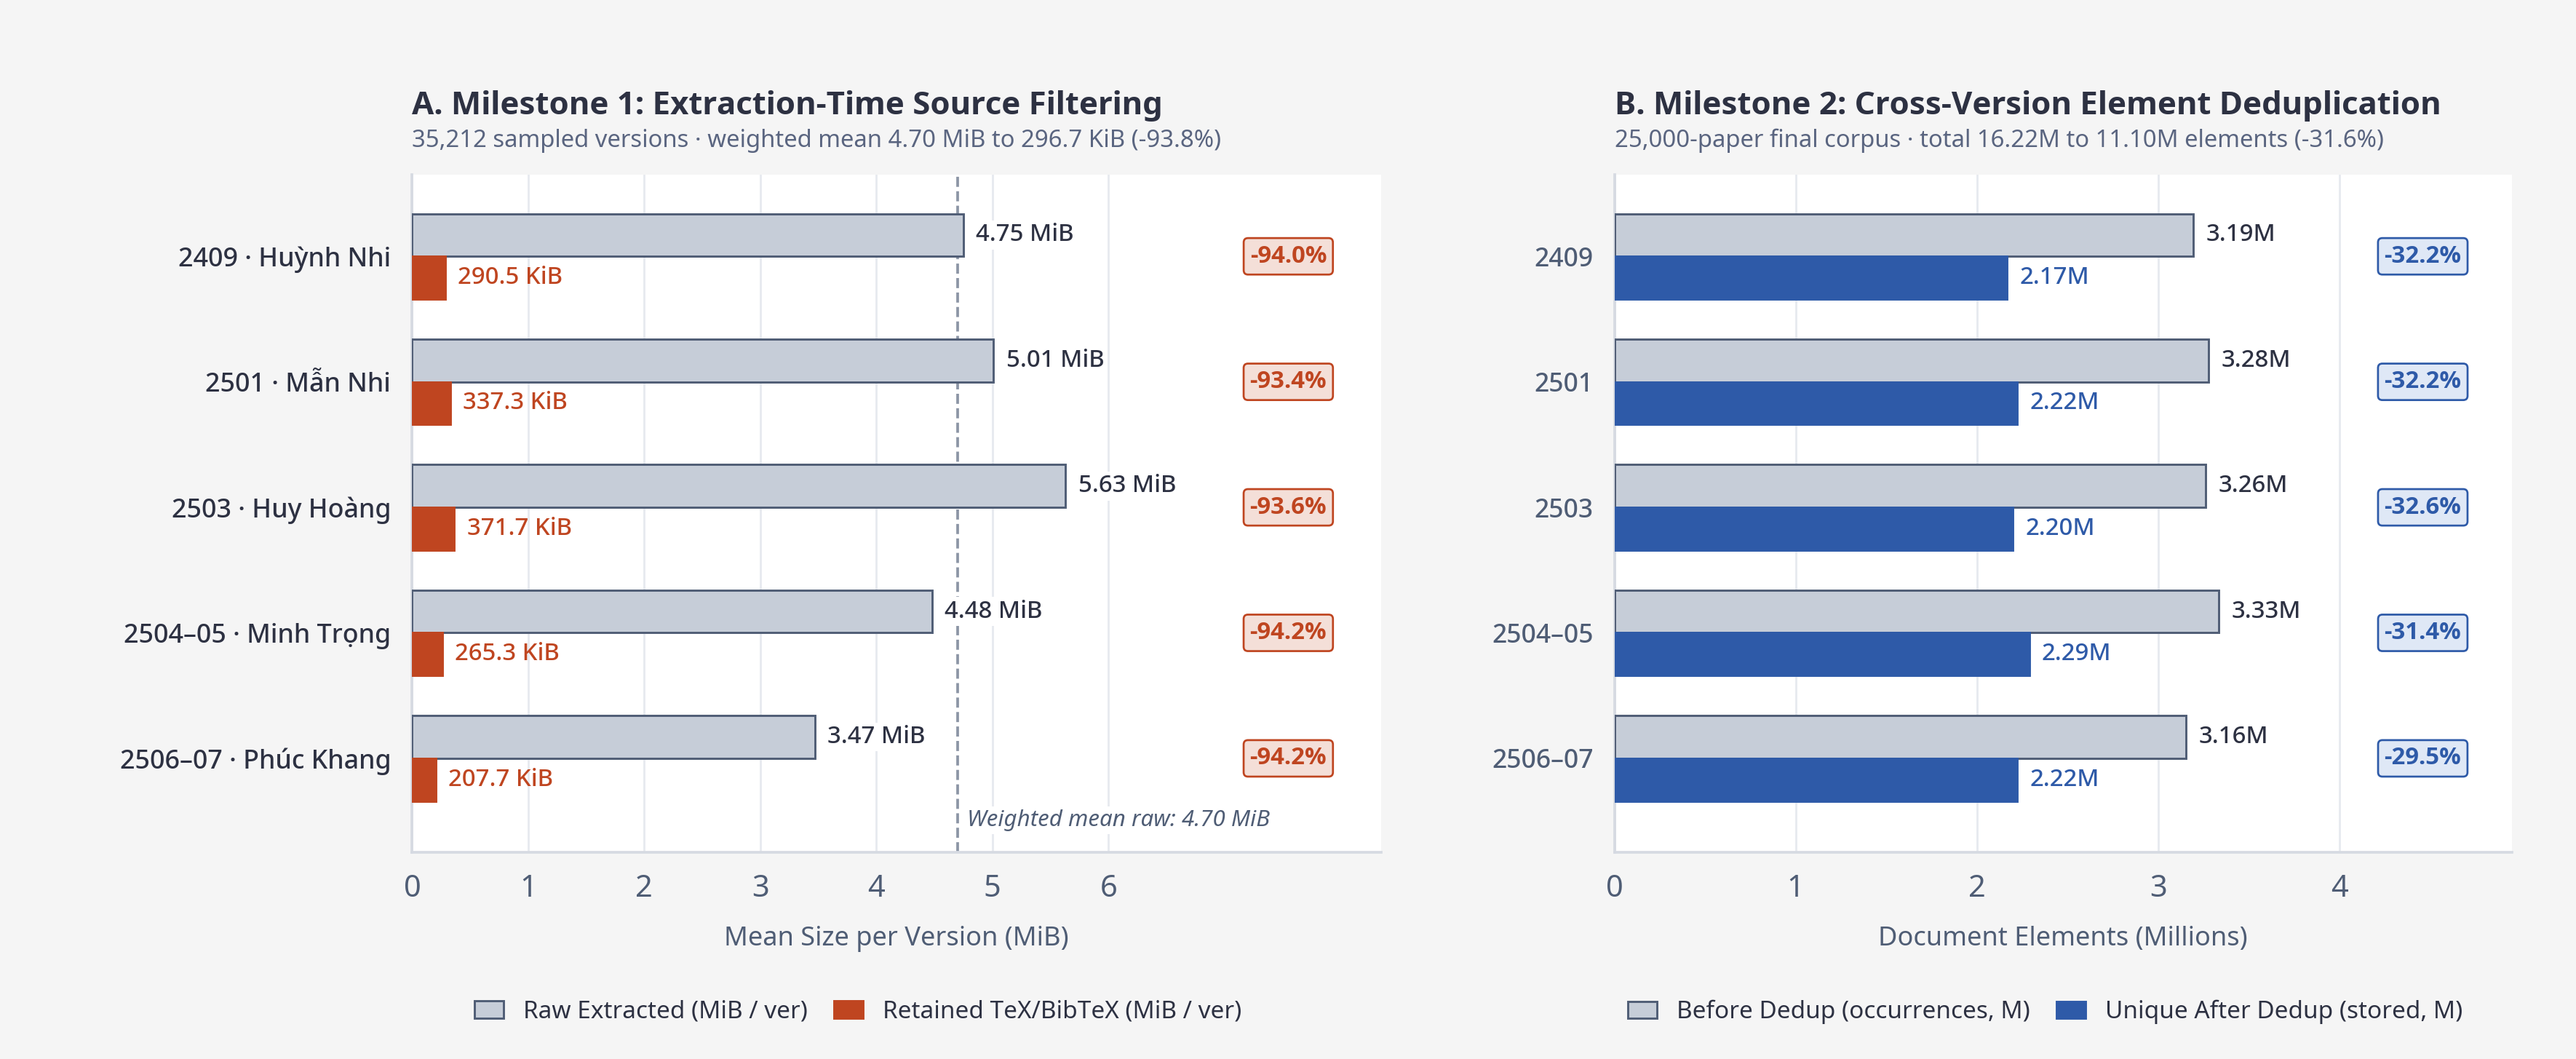
\includegraphics[width=\linewidth]{images/m1_m2_stats.png}
    \caption[Hiệu quả nén dữ liệu tích lũy ở Giai đoạn 1 và khử trùng lặp ở Giai đoạn 2]{Hiệu quả kỹ thuật dữ liệu tích lũy qua hai giai đoạn trên năm dải dữ liệu: mức nén dung lượng nguồn chọn lọc ở Giai đoạn 1 ($-93.83\%$ trên $35{,}212$ phiên bản mẫu) và tỷ lệ khử trùng lặp phần tử nội dung liên phiên bản ở Giai đoạn 2 ($-31.59\%$, từ $16.22$ triệu xuống $11.10$ triệu phần tử duy nhất).}
    \label{fig:m1_m2_stats}
\end{figure}

Về minh bạch số liệu thực nghiệm, cần ghi nhận rõ rằng nhật ký thời gian thực thi tổng thể và bộ nhớ đỉnh trên Google Colab CPU của lượt chạy sản xuất $25{,}000$ bài báo Giai đoạn 2 hiện được lưu trên kho sao lưu đám mây bên ngoài bản chụp cục bộ của dự án. Do không đưa các con số thiếu bản ghi kiểm chứng cục bộ vào báo cáo, toàn bộ phân tích định lượng về tốc độ xử lý, bộ nhớ tiến trình và khả năng mở rộng CPU của Giai đoạn 2 đều căn cứ chặt chẽ vào hai phép đo cục bộ tái lập hoàn toàn trong Bảng~\ref{tab:m2_tokenizer_study}. Trên hạ tầng Colab vốn dễ bị thu hồi máy ảo đột ngột, quy trình vận hành sản xuất bảo vệ tiến độ bằng cơ chế lưu điểm phục hồi quan hệ cục bộ sau từng bài báo. Song song đó, hệ thống định kỳ đồng bộ các thế hệ sao chụp bất biến ra kho lưu trữ ngoài kèm kiểm tra mã băm SHA-256 và đối chiếu dấu vân tay mã nguồn lẫn dữ liệu đầu vào trước khi đóng gói. Ba bảng Parquet đạt chuẩn kiểm định toàn vẹn cuối cùng trở thành nền dữ liệu sạch, thống nhất khóa trích dẫn và sẵn sàng cho bài toán học máy đối sánh tài liệu tham khảo ở Giai đoạn 3.
